\documentclass[12pt]{article}
\usepackage[pdftex]{graphicx}
\usepackage[final]{pdfpages}
\usepackage{svg}
\usepackage{cite} 
\usepackage[german,english]{babel}
\usepackage[round]{natbib}
\setlength{\parindent}{0pt}
\usepackage[onehalfspacing]{setspace} 
\begin{document}
\bibliographystyle{unsrtnat}
\begin{titlepage}

\begin{center}


\includegraphics[width=0.15\textwidth]{./logoTUBerlin}\\[1cm]    

\textsc{\LARGE Technische Universit\"at Berlin}\\[1.5cm]
\textsc{\Large Report}\\[0.2cm]
\textsc{ Advanced Information Management III: Scalable Data Analytics and Data Mining}\\[0.5cm]


\newcommand{\HRule}{\rule{\linewidth}{0.5mm}}
\HRule \\[0.4cm]

{ \Large \bfseries A Comparison of Online learning Na\"ive Bayes Classifier on RSS Feeds using SPARK}\\[0.4cm]

\HRule \\[1.5cm]

\begin{flushleft} \large
\emph{Authors:}\\
Ahmet Anil \textsc{Pala}\\
Franziska \textsc{Adler}
\end{flushleft}

\vfill

{\large \today}

\end{center}

\end{titlepage}
\renewcommand{\contentsname}{Table of Contents}
\tableofcontents

\newpage



\section{Theory}
\subsection{Motivation}
%write here
%example citation: texttexttext\citep[p. 4]{mueller2000}
\begin{spacing}{1.2}
In Text Classification Na\"ive Bayes Classifiers are popular due to their simplicity and find application in the field of spam email detection and descovery of specified web content \citep[p. 225]{ertel2008}. Classifier aim the prediction of a categorie like spam or ham on the basis of previous examples. This can be easily realized with a probalistic classifier like Na\"ive Bayes assuming that the data distribution is static over time, all data is always accessible and query time does not play a major role. For adapting real world problems and their dynamics this might not be sufficient. The developement of the internet and the need of processing huge amounts of available data and answering queries in time-critical situations needs to be taken in account for handeling model construction and model updating. In Online Machine Learning different methods for dealing with sequentially arriving data and updating the model with new incoming observations exist. This is called "Concept Drift" and referes to the problem of the variation of statistical properties \citep{astudillo2013}. Also aspects of scalability might to be considered since Concept Drift occurs mainly in situations of large data qantities arriving via stream \citep[p. 4]{tsymbal2004} and the underlying data processing system is distibuted.   

In this report we are using RSS feeds from BCC for classification on a distributed system. Focus is the evaluation of several Na\"ive Bayes classifiers which implement the online learning paradigm by using streaming techniques.  The evalutation concentrates on the handling of Concept Drift. In a first theoretically part of this report challanges, concepts and methods as well as evaluation measures are described. The second part consits of the explanation of our implementation using SPARK to show how the different classifiers work. Furthermore the evaluation of their performances are analysed and presented.

\end{spacing}

\subsection{Challanges/ Concepts}
%write here
texttexttext

\subsubsection{Concept Drift}
%write here
texttexttext

\subsubsection{Streaming}
%write here
texttexttext

\subsubsection{Distributed Systems}
%write here
Large amounts of data, processing algorithms, ML intense calculation, single machine many nodes, query distribution vs. the other one, HDFS split partitions,  distributed algorithms  

\subsection{Methods}
\subsubsection{Sliding Window}
%write here
texttexttext

\subsection{Evaluation Measurse}
%write here
texttexttext

\section{Empirics}
\subsection{Data}
%write here
texttexttext

\subsection{Software}
%write here
For realising the stated approaches we are using Apache Spark and MLlib. Apache Spark is a open source processing engine for parallel processing of large scale data.   


\subsection{Data}
%write here
texttexttext

\newpage
\subsection{Implementation}
%write here

\begin{figure}[htbp]
  \centering
  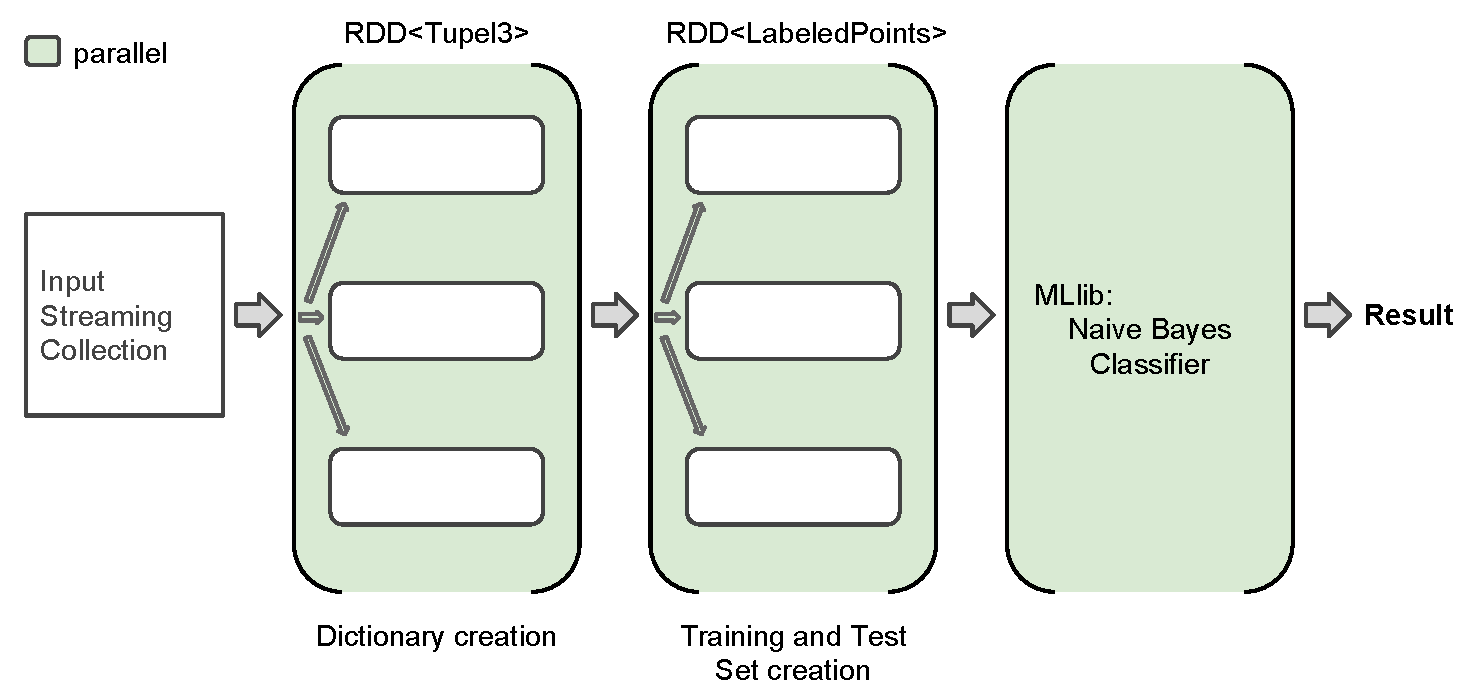
\includegraphics[scale=0.56]{VisualisationOfflineWorkflow.pdf}
  \caption{Offline Workflow}
\end{figure}

\subsection{Evaluation}
%write here
texttexttext

\subsection{Results}
%write here
texttexttext

\subsection{Summary}
%write here
texttexttext




\newpage
\medskip
\bibliography{literatureDB}
\end{document}
